\section{Superficies Paramétricas}

\begin{definición} [Superficie Paramétrica]
Una  parametrización de una superficie paramétrica $S$ en $\mathbb{R}^3$ es una aplicación $\varphi: U \to \mathbb{R}^3$ de clase $C^1$ definida en un abierto conexo $U \subset \mathbb{R}^2$ tal que:
$$ Im(\varphi) = \{ \varphi(u,v) \in \mathbb{R}^3 : (u,v) \in U \} = S $$
Diremos que la parametrización $\varphi$ es regular cuando la pareja de vectores $\left\{\frac{\partial \varphi}{\partial u}, \frac{\partial \varphi}{\partial v}\right\}$ es linealmente independiente en todo punto de $U$. Equivalentemente, cuando el vector normal asociado a $\varphi$ es no nulo en todo punto de $U$:
$$ \vec{N}_{\varphi} = \frac{\partial \varphi}{\partial u} \times \frac{\partial \varphi}{\partial v} \neq \vec{0} $$
En este caso, el plano tangente a la superficie en el punto $\varphi(u_0,v_0)$ tiene como ecuaciones paramétricas:
$$
    \begin{cases}
        x = \varphi_1(u_0,v_0) + \lambda \frac{\partial \varphi_1}{\partial u}(u_0,v_0) + \mu \frac{\partial \varphi_1}{\partial v}(u_0,v_0) \\
        y = \varphi_2(u_0,v_0) + \lambda \frac{\partial \varphi_2}{\partial u}(u_0,v_0) + \mu \frac{\partial \varphi_2}{\partial v}(u_0,v_0) \\
        z = \varphi_3(u_0,v_0) + \lambda \frac{\partial \varphi_3}{\partial u}(u_0,v_0) + \mu \frac{\partial \varphi_3}{\partial v}(u_0,v_0) \\
    \end{cases} \qquad \lambda, \mu \in \mathbb{R}
$$
\end{definición}

\ejemplo{
    Dada la superficie $z=x^2+y^2$, podemos parametrizarla con $\varphi:\mathbb{R}^2 \to \mathbb{R}^3$ dada por $\varphi(x,y) = (x,y,x^2+y^2)$. Calculemos el vector normal:
    $$ \vec{N}_{\varphi} = \frac{\partial \varphi}{\partial x} \times \frac{\partial \varphi}{\partial y} =  \begin{vmatrix}
            \vec{e}_1                             & \vec{e}_2                             & \vec{e}_3                             \\
            \frac{\partial \varphi_1}{\partial x} & \frac{\partial \varphi_2}{\partial x} & \frac{\partial \varphi_3}{\partial x} \\
            \frac{\partial \varphi_1}{\partial y} & \frac{\partial \varphi_2}{\partial y} & \frac{\partial \varphi_3}{\partial y} \\
        \end{vmatrix} = \begin{vmatrix}
            \vec{e}_1 & \vec{e}_2 & \vec{e}_3 \\
            1         & 0         & 2x        \\
            0         & 1         & 2y        \\
        \end{vmatrix} = \vec{e}_1 - 2x\vec{e}_3 + 2y\vec{e}_2 \neq (0,0,0)
    $$}

\ejemplo{
    \underline{Superficies explícitas:} Sean $U \subset \mathbb{R}^2$ abierto conexo y $f: U \to \mathbb{R}$ de clase $C^1$. Entonces la gráfica de $f$ es una superficie regular con parametrización $\varphi: U \to \mathbb{R}^3$ dada por $\varphi(x,y) = (x,y,f(x,y))$.\\
    Veamos que $\vec{N}_{\varphi} \neq (0,0,0)$:
    $$ \vec{N}_\varphi = \frac{\partial \varphi}{\partial x} \times \frac{\partial \varphi}{\partial y} = \begin{vmatrix}
            \vec{e}_1                             & \vec{e}_2                             & \vec{e}_3                             \\
            \frac{\partial \varphi_1}{\partial x} & \frac{\partial \varphi_2}{\partial x} & \frac{\partial \varphi_3}{\partial x} \\
            \frac{\partial \varphi_1}{\partial y} & \frac{\partial \varphi_2}{\partial y} & \frac{\partial \varphi_3}{\partial y} \\
        \end{vmatrix} = \begin{vmatrix}
            \vec{e}_1 & \vec{e}_2 & \vec{e}_3                     \\
            1         & 0         & \frac{\partial f}{\partial x} \\
            0         & 1         & \frac{\partial f}{\partial y} \\
        \end{vmatrix} = \vec{e}_1 - \frac{\partial f}{\partial x}\vec{e}_3 + \frac{\partial f}{\partial y}\vec{e}_2 \neq (0,0,0)
    $$
    $$ Im(\varphi) = \{(x,y,z) \in \mathbb{R}^3 : (x,y) \in U, z = f(x,y)\} $$
}

\ejemplo{
    Dado el cilindro de ecuaciones $x^2 + y^2 = 1, \ 0 < z < 1$, buscamos una parametrización de la superficie.\\
    Tomando la siguiente parametrización:
    $$
        \begin{cases}
            x = \cos(\theta) \\
            y = \sin(\theta) \\
            z = z
        \end{cases} \qquad \theta \in \mathbb{R}, \quad z \in (0,1)
    $$
    entonces vemos que $\underbrace{x^2 + y^2}_{1} = r^2 \implies r = 1$.\\
    Por tanto, obtenemos que nuestra parametrización es:
    $$ \varphi : \mathbb{R} \times (0,1) \to \mathbb{R}^3 \quad \varphi(\theta,z) = (\cos(\theta),\sin(\theta),z) $$
    Calculemos el vector normal:
    $$ \vec{N}_{\varphi} = \begin{vmatrix}
            \vec{e}_1                                  & \vec{e}_2                                  & \vec{e}_3                                  \\
            \frac{\partial \varphi_1}{\partial \theta} & \frac{\partial \varphi_2}{\partial \theta} & \frac{\partial \varphi_3}{\partial \theta} \\
            \frac{\partial \varphi_1}{\partial z}      & \frac{\partial \varphi_2}{\partial z}      & \frac{\partial \varphi_3}{\partial z}      \\
        \end{vmatrix} = \begin{vmatrix}
            \vec{e}_1     & \vec{e}_2    & \vec{e}_3 \\
            -\sin(\theta) & \cos(\theta) & 0         \\
            0             & 0            & 1         \\
        \end{vmatrix} = (\cos(\theta),\sin(\theta),0) \neq (0,0,0)
    $$
}

\ejemplo{
    Tomando el cilindro $x^2 + y^2 = 1, \ 0 < z < 1$ del ejemplo anterior, podemos parametrizarlo de otra forma.\\
    Consideramos el siguiente conjunto:
    $$ U = \{ (u,v) : 1 < \sqrt{u^2 + v^2} < 2, \quad 0 < v < 2\pi \} $$
    entonces definimos nuestra parametrización $\varphi: U \to \mathbb{R}^3$ sobre este conjunto tal que
    $$\varphi(u,v) = \left(\frac{u}{\sqrt{u^2 + v^2}}, \frac{v}{\sqrt{u^2 + v^2}}, \sqrt{u^2 + v^2}-1\right) $$
}

\begin{definición} [Superficies Equivalentes] Diremos que dos superficies paramétricas \( \varphi: U \to \mathbb{R}^3 \) y \( \psi: V \to \mathbb{R}^3 \), definidas respectivamente sobre los conjuntos abiertos conexos \( U, V \subset \mathbb{R}^2 \), son equivalentes si existe una aplicación biyectiva \( h: V \to U \) de clase \( C^1 \) (es decir, un difeomorfismo) tal que: \[ \psi = \varphi \circ h. \]
\end{definición}

\begin{observación}
\vspace{-2.5em}
\begin{enumerate}
    \item En este caso $\varphi(U) = \psi(V)$.
    \item En la definición se pide que los conjuntos $U$ y $V$ sean conexos. Como
          $\forall (s,t) \in V$, $D_h(s,t) : \mathbb{R}^2 \to \mathbb{R}^2$ es un
          isomorfismo lineal, sabemos que $det(D_h(s,t)) \neq 0$. Por conexión,
          $det(D_h(s,t))$ conserva el signo en todo $V$.
\end{enumerate}
\end{observación}

\begin{definición} [Conservación de la Orientación]
\vspace{-2.5em}
\begin{enumerate}
    \item Se dice que $h$ conserva la orientación si $det(D_h(s,t)) > 0$ para todo $(s,t)
              \in V$, es decir las funciones $\varphi$ y $\psi$ tienen la misma orientación.
    \item Se dice que $h$ cambia la orientación si $det(D_h(s,t)) < 0$ para todo $(s,t)
              \in V$, es decir las funciones $\varphi$ y $\psi$ tienen orientaciones
          opuestas.
\end{enumerate}
\end{definición}

\begin{lema}
    Sean \( \varphi: U \to \mathbb{R}^3 \) y \( \psi: V \to \mathbb{R}^3 \) dos parametrizaciones equivalentes de una superficie \( S \). Entonces, para todo \( (s,t) \in V \), se cumple que:
    \[
        \frac{\partial \psi}{\partial s} \times \frac{\partial \psi}{\partial t} = det(D_h(s,t)) \cdot \frac{\partial \varphi}{\partial u} \times \frac{\partial \varphi}{\partial v} (h(s,t))
    \]
    Equivalentemente,
    \[
        \vec{N}_{\psi} (s,t) = det(D_h(s,t)) \cdot \vec{N}_{\varphi}(h(s,t))
    \]
\end{lema}

\begin{proof}
    Aplicando la regla de la cadena a \(\psi = \varphi \circ h\), obtenemos la siguiente relación entre las matrices jacobianas:
    \[
        D_\psi(s,t) = D_\varphi(h(s,t)) \cdot D_h(s,t).
    \]
    En términos de las derivadas parciales, esto se traduce en:
    \[
        \frac{\partial \psi}{\partial s} = \frac{\partial \varphi}{\partial u} \frac{\partial h_1}{\partial s} + \frac{\partial \varphi}{\partial v} \frac{\partial h_2}{\partial s}, \quad \frac{\partial \psi}{\partial t} = \frac{\partial \varphi}{\partial u} \frac{\partial h_1}{\partial t} + \frac{\partial \varphi}{\partial v} \frac{\partial h_2}{\partial t},
    \]
    donde \(h(s,t) = (h_1(s,t), h_2(s,t))\).

    Podemos escribir estas ecuaciones en forma matricial como:
    \[
        \left( \frac{\partial \psi}{\partial s}, \frac{\partial \psi}{\partial t} \right) = \left( \frac{\partial \varphi}{\partial u}, \frac{\partial \varphi}{\partial v} \right) \cdot D_h(s,t),
    \]
    donde \(D_h(s,t)\) es la matriz jacobiana de \(h\):
    \[
        D_h(s,t) = \begin{pmatrix}
            \frac{\partial h_1}{\partial s} & \frac{\partial h_1}{\partial t} \\
            \frac{\partial h_2}{\partial s} & \frac{\partial h_2}{\partial t}
        \end{pmatrix}.
    \]

    Ahora, consideremos el producto vectorial de las derivadas parciales de
    \(\psi\):
    \[
        \frac{\partial \psi}{\partial s} \times \frac{\partial \psi}{\partial t}.
    \]
    Utilizando las expresiones anteriores, tenemos:
    \[
        \frac{\partial \psi}{\partial s} \times \frac{\partial \psi}{\partial t} = \left( \frac{\partial \varphi}{\partial u} \frac{\partial h_1}{\partial s} + \frac{\partial \varphi}{\partial v} \frac{\partial h_2}{\partial s} \right) \times \left( \frac{\partial \varphi}{\partial u} \frac{\partial h_1}{\partial t} + \frac{\partial \varphi}{\partial v} \frac{\partial h_2}{\partial t} \right).
    \]
    Expandiendo el producto vectorial y usando que \(\frac{\partial
        \varphi}{\partial u} \times \frac{\partial \varphi}{\partial u} = 0\) y
    \(\frac{\partial \varphi}{\partial v} \times \frac{\partial \varphi}{\partial
        v} = 0\), obtenemos:
    \[
        \frac{\partial \psi}{\partial s} \times \frac{\partial \psi}{\partial t} = \left( \frac{\partial h_1}{\partial s} \frac{\partial h_2}{\partial t} - \frac{\partial h_1}{\partial t} \frac{\partial h_2}{\partial s} \right) \left( \frac{\partial \varphi}{\partial u} \times \frac{\partial \varphi}{\partial v} \right).
    \]
    Notamos que el término entre paréntesis a la derecha es el determinante de la
    matriz jacobiana \(D_h(s,t)\):
    \[
        \det(D_h(s,t)) = \frac{\partial h_1}{\partial s} \frac{\partial h_2}{\partial t} - \frac{\partial h_1}{\partial t} \frac{\partial h_2}{\partial s}.
    \]
    Por lo tanto, hemos demostrado que:
    \[
        \frac{\partial \psi}{\partial s} \times \frac{\partial \psi}{\partial t} = \det(D_h(s,t)) \cdot \left( \frac{\partial \varphi}{\partial u} \times \frac{\partial \varphi}{\partial v} \right)(h(s,t)).
    \]
    Equivalentemente, para los vectores normales unitarios:
    \[
        \vec{N}_{\psi}(s,t) = \det(D_h(s,t)) \cdot \vec{N}_{\varphi}(h(s,t)),
    \]
    donde \(\vec{N}_{\psi}\) y \(\vec{N}_{\varphi}\) son los vectores normales
    unitarios asociados a las parametrizaciones \(\psi\) y \(\varphi\),
    respectivamente.
\end{proof}

\begin{definición} [Orientación de una Superficie]
Asociadas a las parametrizaciones $\varphi$ y $\psi$ obtenemos lso vectores normales unitarios
$$ \vec{n}_{\varphi} = \frac{\vec{N}_{\varphi}}{||\vec{N}_{\varphi}||} \quad \text{y} \quad \vec{n}_{\psi} = \frac{\vec{N}_{\psi}}{||\vec{N}_{\psi}||} $$
Entonces diremos que $\varphi$ y $\psi$ tienen la misma orientación si:
$$ \vec{n}_{\psi} (s,t) = \vec{n}_{\varphi}(h(s,t)) \text{  o  } \vec{n}_{\psi} (s,t) = -\vec{n}_{\varphi}(h(s,t)) $$
\end{definición}

\subsection{Superficies como Conjuntos}

\begin{definición} [Superficie Simple Regular]
Diremos que $S \subset \mathbb{R}^3$ es una superficie simple regular si $S = \varphi (\overline{D})$ donde $\overline{D} = Int(C)$ siendo $C \subset \mathbb{R}^2$ una curva de Jordan regular a trozos, y $\varphi: U \to \mathbb{R}^3$ una parametrización de clase $C^1$ inyectiva y regular en $\overline{D}$.\\
En este caso, se dice que la curva $\varphi(C)$ es el borde de $S$. Así, $\gamma = \varphi(C)$ es una curva cerrada y regular a trozos en $\mathbb{R}^3$.
\end{definición}

\begin{definición} [Superficie Casi-Simple Regular]
Diremos que $S \subset \mathbb{R}^3$ es una superficie casi-simple regular si $S = \varphi (\overline{D})$ donde $\overline{D} = Int(C)$ siendo $C \subset \mathbb{R}^2$ una curva de Jordan regular a trozos, y $\varphi: U \to \mathbb{R}^3$ una parametrización de clase $C^1$ inyectiva y regular en $D$.
\end{definición}

\begin{definición}
Dada una superficie $S$ en $\mathbb{R}^3$ simple regular o casi-simple regular, y una parametrización $\varphi: U \to \mathbb{R}^3$ de clase $C^1$ de $S$, definimos:
\vspace{-0.5em}
\begin{enumerate}
    \item El área de la superficie $S$ como: $$ a(S) = \int_{D} \left\lVert
              \frac{\partial \varphi}{\partial u} \times \frac{\partial \varphi}{\partial v}
              \right\rVert dudv $$
    \item  Si $f: S \to \mathbb{R}$ es una función continua, entonces la integral de
          superficie de $f$ sobre $S$ es: $$ \int_{S} f dS = \int_{D} f(\varphi(u,v))
              \left\lVert \frac{\partial \varphi}{\partial u} \times \frac{\partial
                  \varphi}{\partial v} \right\rVert dudv $$
\end{enumerate}
\end{definición}

\ejemplo{
Consideramos la superficie $S$ de $\mathbb{R}^3$ resultante de acotar un cono por dos planos paralelos al plano $XY$, y dada por las ecuaciones:
$$S = \{(x,y,z) \in \mathbb{R}^3 : x^2 + y^2 = z^2, \ 1 < z < 2\}$$
Calculemos el área de la superficie $S$:\\
$$
    \begin{cases}
        x = r \cos(\theta) \\
        y = r \sin(\theta) \\
        z = r
    \end{cases} \qquad r^2 = x^2 + y^2 = z^2 \implies r = z \qquad \varphi(\theta,z) = \begin{cases}
        x = z \cos(\theta) \\
        y = z \sin(\theta) \\
        z = z
    \end{cases}
$$
$$\overline{D} =[0,2\pi] \times [1,2] \qquad S = \varphi(D)$$
$$ \vec{N}_\varphi = \begin{vmatrix}
        \vec{e}_1      & \vec{e}_2     & \vec{e}_3 \\
        -z\sin(\theta) & z\cos(\theta) & 0         \\
        \cos(\theta)   & \sin(\theta)  & 1
    \end{vmatrix} = (z\cos(\theta), z\sin(\theta), -z)
$$
$$ \lVert \vec{N}_\varphi \rVert^2 = z^2\cos^2(\theta) + z^2\sin^2(\theta) + (-z)^2 = 2z^2 \implies \lVert \vec{N}_\varphi \rVert = z\sqrt{2} \neq 0 \quad \forall (0,z) \in D $$
Entonces $\varphi$ es inyectiva y regular en $D$ (aunque no en $\overline{D}$), luego $S$ es una superficie casi-simple regular.\\
Por último, el área de la superficie $S$ es:
$$ a(S) = \int_{D} \lVert \vec{N}_\varphi \rVert dudv = \int_{\theta = 0}^{\theta = 2\pi} \int_{z = 1}^{z = 2} z\sqrt{2} dz d\theta = \int_{\theta = 0}^{\theta = 2\pi} \left[ \frac{z^2}{2}\sqrt{2} \right]_{1}^{2} d\theta $$
$$= \int_{\theta = 0}^{\theta = 2\pi} \left( \frac{4}{2}\sqrt{2} - \frac{1}{2}\sqrt{2} \right) d\theta = \int_{\theta = 0}^{\theta = 2\pi} \frac{3}{2}\sqrt{2} d\theta = \frac{3}{2}\sqrt{2} \cdot 2\pi = 3\pi\sqrt{2}$$
}

\ejemplo{
    Dada la función $f(x,y,z) = x^2 + y^2 + z^2$, calculemos la integral de superficie de $f$ sobre la superficie $S$ dada por la sección de cono $x^2 + y^2 = z^2, \ 1 < z < 2$ del ejemplo anterior.\\
    Entonces, la integral de superficie de $f$ sobre $S$ es:
    $$ \int_{S} f dS = \int_{D} f(\varphi(\theta,z)) \lVert \vec{N}_\varphi \rVert d\theta dz = \int_{\theta = 0}^{\theta = 2\pi} \int_{z = 1}^{z = 2} 2z^2 \cdot z\sqrt{2} dz d\theta = \int_0^{2\pi} \frac{2\sqrt{2}}{4} \left[ z^4 \right]_1^2 \, d\theta $$
    $$= \int_0^{2\pi} \frac{2\sqrt{2}}{4} (16 - 1) \, d\theta = \int_0^{2\pi} \frac{30\sqrt{2}}{4} \, d\theta = \int_0^{2\pi} \frac{15\sqrt{2}}{2} \, d\theta = \frac{15\sqrt{2}}{2} \cdot (2\pi) = 15\pi\sqrt{2}$$
    Observemos que $\int_{S} f dA = \int_{S} f dS$.
}

\ejemplo{
    Area de una esfera en $\mathbb{R}^3$:\\
    $$ S_R = \{(x,y,z) \in \mathbb{R}^3 : x^2 + y^2 + z^2 = R^2\} \quad R>0$$
    Sea:
    $$ \varphi \begin{cases}
        x = R \cos(\theta) \sin(\psi) \\
        y = R \sin(\theta) \sin(\psi) \\
        z = R \cos(\psi)
    \end{cases} 
    \qquad 
    \left( \begin{matrix}
        0 \leq \theta \leq 2\pi \\
        0 \leq \psi \leq \pi 
    \end{matrix} \right)
    \equiv \overline{D}$$
    Ahora calculemos $\vec{N}_\varphi$:
    $$ \vec{N}_\varphi = \begin{vmatrix}
        \vec{e}_1 & \vec{e}_2 & \vec{e}_3 \\
        -R\sin(\theta)\sin(\psi) & R\cos(\theta)\sin(\psi) & 0 \\
        R\cos(\theta)\cos(\psi) & R\sin(\theta)\cos(\psi) & -R\sin(\psi)
    \end{vmatrix}
    =$$
    $$\left( -R^2\cos(\theta)\sin^2(\psi), -R^2\sin(\theta)\sin^2(\psi), -R^2cos(\psi)\sin(\psi) \right)$$
    Ahora deducimos:
    $$ \lVert \vec{N}_\varphi \rVert^2 = R^4 \sin^4(\psi) + R^4 \cos^2(\psi)\sin^2(\psi) = R^4 \sin^2(\psi)\\
    \implies \lVert \vec{N}_\varphi \rVert = R^2 \sin(\psi)$$ 
    Finalmente calculemos el area:
    $$area(S_R) = \int_{D} \lVert \vec{N}_\varphi \rVert = \int_{\theta = 0}^{\theta = 2\pi} \int_{\psi = 0}^{\psi = \pi} R^2 \sin(\psi) R^2 \sin(\psi) d\psi d\theta = 2\pi R^2 \left[ -\cos(\psi) \right]_{\psi = 0}^{\psi = \pi} = 4\pi R^2$$
}

\begin{definición}[Superficies Regulares a trozos (suma de superficies)]
    Sean $S_1, S_2 \subset \mathbb{R}^3$ dos superficies simples regulares. Se dice que $S$ es la suma de $S_1$ y $S_2$ y denotamos $S = S_1 + S_2$ cuando:\\
    \begin{enumerate}
        \item $S = S_1 \cup S_2$.
        \item $S_1 \cap S_2 = \partial S_1 \cap \partial S_2$.
    \end{enumerate}
    En este caso se define el borde de $S$ como
    $$ \partial S = \overline{ \left( \partial S_1 \cup \partial S_2 \right) \setminus \left(\partial S_1 \cap \partial S_2 \right) } $$
    Si $\partial S = \emptyset$ se dice que $S$  no tiene botde y es cerrada.\\

    Analogamente podemos definir la suma de superficies $S_1 + S_2 + \ldots + S_k$ siendo cada $S_i \quad i \in [1,k]$ una superficie simple regular.\\
\end{definición}

\ejemplo{
    Superficie del cubo
    $$ S = S_1 + S_2 + S_3 + S_4 + S_5 + S_6, \qquad \partial S = \emptyset $$
    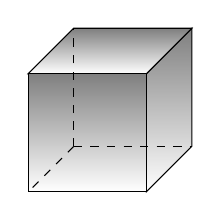
\begin{tikzpicture}[scale=1.5]
        % Caras visibles
        \draw[shade] (1,0,0) -- (1,1,0) -- (1,1,1) -- (1,0,1) -- cycle;
        \draw[shade] (0,1,0) -- (0,1,1) -- (1,1,1) -- (1,1,0) -- cycle;
        \draw[shade] (0,0,1) -- (1,0,1) -- (1,1,1) -- (0,1,1) -- cycle;
        % Lineas traseras
        \draw[dashed] (0,0,0) -- (1,0,0);
        \draw[dashed] (0,0,0) -- (0,1,0);
        \draw[dashed] (0,0,0) -- (0,0,1);
    \end{tikzpicture}
}

\ejemplo{
    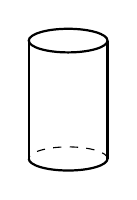
\begin{tikzpicture}[scale=0.5]
        % Cilindro
        \draw[thick] (0,0) ellipse (1 and 0.3);
        \draw[thick] (-1,0) -- (-1,-3);
        \draw[thick] (1,0) -- (1,-3);
        \draw[thick] (-1,-3) arc (180:360:1 and 0.3);
        \draw[dashed] (1,-3) arc (0:180:1 and 0.3);
    \end{tikzpicture}
}